%% LyX 2.2.1 created this file.  For more info, see http://www.lyx.org/.
%% Do not edit unless you really know what you are doing.
\documentclass[english,12pt]{article}
\usepackage[T1]{fontenc}
\usepackage[latin9]{inputenc}
\usepackage{mathtools}
\usepackage{amsmath}
\usepackage{amsthm}
\usepackage{amssymb}
\usepackage{graphicx}
\PassOptionsToPackage{normalem}{ulem}
\usepackage{ulem}

\makeatletter
%%%%%%%%%%%%%%%%%%%%%%%%%%%%%% Textclass specific LaTeX commands.
\theoremstyle{plain}
\newtheorem{thm}{\protect\theoremname}[section]
\theoremstyle{plain}
\newtheorem{prop}[thm]{\protect\propositionname}
\ifx\proof\undefined
\newenvironment{proof}[1][\protect\proofname]{\par
\normalfont\topsep6\p@\@plus6\p@\relax
\trivlist
\itemindent\parindent
\item[\hskip\labelsep\scshape #1]\ignorespaces
}{%
\endtrivlist\@endpefalse
}
\providecommand{\proofname}{Proof}
\fi
\theoremstyle{definition}
\newtheorem{example}[thm]{\protect\examplename}
\theoremstyle{definition}
\newtheorem{defn}[thm]{\protect\definitionname}

%%%%%%%%%%%%%%%%%%%%%%%%%%%%%% User specified LaTeX commands.
\usepackage[margin=1in]{geometry}

\makeatother

\usepackage{babel}
\providecommand{\definitionname}{Definition}
\providecommand{\examplename}{Example}
\providecommand{\propositionname}{Proposition}
\providecommand{\theoremname}{Theorem}

\begin{document}

\title{Math 525: Lecture 12}

\date{February 13, 2018}
\maketitle

\section{Moment generating functions (a rigorous treatment)}

Remember the moment generating function of a random variable $X$?
It looked like
\[
M(\theta)=\mathbb{E}\left[e^{\theta X}\right].
\]
A few lectures ago, we worked on the theory of limits of expectations
(Monotone Convergence Theorem, Fatou's Lemma, Dominated Convergence
Theorem) with the motivation of being able to rigorously treat moment
generating functions. Let's do that now.
\begin{prop}
Suppose $M(\theta)$ is well-defined in a neighbourhood of the origin.
Then,
\[
M^{(k)}(\theta)=\mathbb{E}[X^{k}e^{\theta X}]
\]
in a neighbourhood of the origin.
\end{prop}
\begin{proof}
We start with the case of $k=1$. By definition,
\begin{align*}
M^{\prime}(\theta) & =\lim_{h\downarrow0}\frac{M(\theta+h)-M(\theta)}{h}\\
 & =\lim_{h\downarrow0}\frac{\mathbb{E}\left[e^{\left(\theta+h\right)X}\right]-\mathbb{E}\left[e^{\theta X}\right]}{h}\\
 & =\lim_{h\downarrow0}\mathbb{E}\left[\frac{e^{\left(\theta+h\right)X}-e^{\theta X}}{h}\right].
\end{align*}
We would like to move the limit inside the expectation to get
\[
\mathbb{E}\left[\lim_{h\downarrow0}\frac{e^{\left(\theta+h\right)X}-e^{\theta X}}{h}\right]=\mathbb{E}\left[\frac{d}{d\theta}e^{\theta X}\right]=\mathbb{E}\left[Xe^{\theta X}\right].
\]
In order to show that this is possible, we will apply the dominated
convergence theorem.

Choose $b>0$ small enough so that $M(\pm b)$ is well-defined. Now,
pick $\epsilon$ such that $0<\epsilon<b$. Assume $\theta$ and $h$
are small enough so that both $\theta$ and $\theta+h$ are in the
interval $(-b+\epsilon,b-\epsilon)$. For each $x$, the mean value
theorem tells us that we can find $\alpha(x)\in(\theta,\theta+h)$
such that 
\[
\frac{e^{(\theta+h)x}-e^{\theta x}}{h}=xe^{\alpha(x)x}.
\]
Note that
\[
\left|xe^{\alpha(x)x}\right|\leq\left|x\right|e^{|\alpha(x)x|}=\left|x\right|e^{(b-\epsilon)|x|}\leq\left|x\right|e^{-\epsilon|x|}e^{b|x|}.
\]
The function $x\mapsto|x|e^{-\epsilon|x|}$ is bounded on the real
line (see Figure \ref{fig:bounded}).
\begin{figure}
\begin{centering}
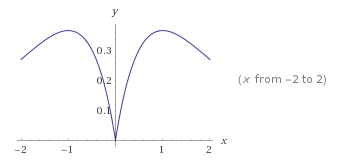
\includegraphics{bounded}
\par\end{centering}
\caption{$x\mapsto|x|e^{-|x|}$\label{fig:bounded}}
\end{figure}
Therefore, we can find some constant $C(\epsilon)$ such that
\[
\left|xe^{\alpha(x)x}\right|\leq C(\epsilon)e^{b|x|}\leq C(\epsilon)\left(e^{bx}+e^{-bx}\right).
\]
Define the random variable $Y$ by
\[
Y=C(\epsilon)\left(e^{bX}+e^{-bX}\right).
\]
The inequalities above show that $Y$ dominates $|X^{\alpha(X)X}|$.
Moreover, $Y$ is integrable since
\[
\mathbb{E}Y=b\left(M(b)+M(-b)\right).
\]
The rest follows by the Dominated Convergence Theorem.

As for the case of $k>1$, we simply apply the argument inductively,
noting that
\[
\frac{d}{d\theta}\left[x^{k-1}e^{\theta x}\right]=x^{k}e^{\theta x}.\qedhere
\]
\end{proof}

\section{Characteristic functions}

Moment generating functions, while very useful, have one big flaw:
their usefulness depends on whether or not they are well-defined on
an interval about the origin. Let's visit an example where the moment
generating function fails this condition:
\begin{example}
The Cauchy distribution (centred at zero) has probability density
function
\[
f(x)=\frac{1}{\pi\gamma}\left(\frac{\gamma^{2}}{(x-x_{0})^{2}+\gamma^{2}}\right)
\]
where $x_{0}$ specifies the peak of the density and $\gamma>0$ is
a scaling parameter. Let's take $x_{0}=0$ and $\gamma=1$ for simplicity.
Let $X$ be a random variable with probability density $f$. In this
case,
\[
M(\theta)=\mathbb{E}\left[e^{\theta X}\right]=\int_{-\infty}^{\infty}e^{\theta x}f(x)dx=\frac{1}{\pi}\int_{-\infty}^{\infty}e^{\theta x}\frac{1}{x^{2}+1}dx.
\]
If $\theta=0$, the above integral becomes $\frac{1}{\pi}\int_{-\infty}^{\infty}\frac{1}{x^{2}+1}dx=1$.
Otherwise, the term $e^{\theta|x|}\frac{1}{x^{2}+1}$ grows quickly
enough as $|x|\rightarrow\infty$ for the integral to diverge.
\end{example}
\begin{figure}
\begin{centering}
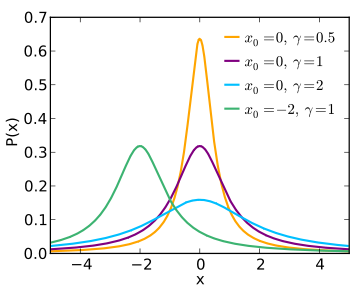
\includegraphics[height=3in]{cauchy}
\par\end{centering}
\caption{Cauchy probability density}
\end{figure}

We want a moment generating function that's valid for all distributions.
This is our motivation today. First, we need the notion of a complex-valued
random variable:
\begin{defn}
Let $U$ and $V$ be real-valued random variables. Then, we call $Z=U+iV$
a \emph{complex-valued random variable}.
\end{defn}
We define $\mathbb{E}Z=\mathbb{E}U+i\mathbb{E}V$ whenever $U$ and
$V$ are integrable. We point out that $|\mathbb{E}Z|\leq\mathbb{E}|Z|$
(in this case, $|\cdot|$ is the modulus of a complex number).
\begin{defn}
The \emph{characteristic function} of a random variable $X$ is given
by
\[
\phi(t)=\mathbb{E}\left[e^{itX}\right].
\]
\end{defn}
Let's prove some properties of the characteristic function.
\begin{prop}
Let $X$ be a random variable and $\phi$ be its characteristic function.
Then,
\begin{enumerate}
\item $\phi(0)=1$ and $|\phi(t)|\leq1$ for all $t$ (namely, the characteristic
function is defined for \uline{all} $t$).
\item $\phi$ is a uniformly continuous function.
\item $\phi(t)$ is positive definite. That is, for all $t_{1},\ldots,t_{n}\in\mathbb{R}$
and $z_{1},\ldots,z_{n}\in\mathbb{C}$,
\[
\sum_{k,j=1}^{n}\phi(t_{k}-t_{j})z_{k}\overline{z_{j}}\geq0.
\]
\end{enumerate}
\end{prop}
\begin{proof}
~
\begin{enumerate}
\item Note that $\phi(0)=\mathbb{E}[e^{i0X}]=1$. As for the other claim
$\mathbb{E}\left[|e^{itX}|\right]\leq1$.
\item Note that
\begin{multline*}
\left|\phi(t+s)-\phi(t)\right|=\left|\mathbb{E}\left[e^{i(t+s)X}-e^{itX}\right]\right|\leq\mathbb{E}\left|e^{itX}\left(e^{isX}-1\right)\right|=\mathbb{E}\left[\left|e^{itX}\right|\left|e^{isX}-1\right|\right]\\
=\mathbb{E}\left|e^{isX}-1\right|.
\end{multline*}
Now, let $\delta(s)=\mathbb{E}|e^{isX}-1|$. Note that $\delta(s)\leq2$
and $\delta(s)\rightarrow0$ as $s\rightarrow0$. In other words,
the right hand side of
\[
\left|\phi(t+s)-\phi(t)\right|\leq\delta(s)
\]
is bounded independently of $t$, from which we obtain the desired
result.
\item The last claim follows from some algebra:
\begin{align*}
\sum_{k,j=1}^{n}\phi(t_{k}-t_{j})z_{k}\overline{z_{j}} & =\mathbb{E}\left[\sum_{k,j=1}^{n}e^{i(t_{k}-t_{j})X}z_{k}\overline{z_{j}}\right]\\
 & =\mathbb{E}\left[\sum_{k,j}e^{it_{k}X}z_{k}e^{-it_{j}X}\overline{z_{j}}\right]\\
 & =\mathbb{E}\left[\sum_{k}\sum_{j}e^{it_{k}X}z_{k}\overline{e^{it_{j}X}z_{j}}\right]\\
 & =\mathbb{E}\left[\left(\sum_{k}e^{it_{k}X}z_{k}\right)\overline{\left(\sum_{j}e^{it_{j}X}z_{j}\right)}\right]\\
 & \geq0.
\end{align*}
\end{enumerate}
\end{proof}
Let's now prove that the characteristic function also generates the
moments by differentiation. In other words, we can think of the characteristic
function as the new and improved ``version 2'' of the MGF.
\begin{prop}
Let $\phi$ be the characteristic function of a random variable $X$.
\begin{enumerate}
\item If $X^{k}$ is integrable, then $\phi$ is $k$ times differentiable.
Moreover,
\begin{equation}
\phi(t)=\sum_{j=0}^{k}\frac{(it)^{j}}{j!}\mathbb{E}[X^{j}]+o(t^{k})\qquad\text{as }t\rightarrow0.\label{eq:taylor}
\end{equation}
In particular,
\[
\phi^{(n)}(0)=i^{n}\mathbb{E}[X^{n}]\qquad\text{for }n=1,\ldots,k.
\]
\item Conversely, if $\phi^{(2k)}(0)$ exists and is finite, then $\mathbb{E}[|X|^{2k}]<\infty$.
\end{enumerate}
\end{prop}
\begin{proof}
~
\begin{enumerate}
\item Our proof is going to be very similar to the proof for the MGF which
we saw earlier. Let's start with $k=1$. Let $h>0$ and consider the
quantity
\begin{align}
\frac{\phi(t+h)-\phi(t)}{h} & =\frac{\mathbb{E}\left[e^{i(t+h)X}-e^{itX}\right]}{h}\nonumber \\
 & =\mathbb{E}\left[e^{itX}\frac{e^{ihX}-1}{h}\right]\label{eq:derivative}
\end{align}
Now, note that
\[
\frac{e^{ihX}-1}{h}=\frac{\cos(hX)-1}{h}+i\frac{\sin(hX)}{h}.
\]
By the mean value theorem, we can find $\theta$ and $\theta^{\prime}$
(depending on $\omega$) between $0$ and $h$ such that
\[
\frac{\cos(hX)-\cos(0X)}{h}=\frac{\cos(hX)-1}{h}=-X\sin(\theta X)
\]
and
\[
\frac{\sin(hX)-\sin(0X)}{h}=\frac{\sin(hX)}{h}=X\cos(\theta^{\prime}X).
\]
Therefore,
\[
\frac{e^{ihX}-1}{h}=-X\sin(\theta X)+X\cos(\theta^{\prime}X)
\]
and hence
\[
\left|\frac{e^{ihX}-1}{h}\right|\leq\left|X\right|\left|\sin(\theta X)+\cos(\theta^{\prime}X)\right|\leq2\left|X\right|.
\]
We have proved that the argument in the expectation (\ref{eq:derivative})
is dominated by an integrable random variable (namely, $2|X|$). Therefore,
we can take limits to get
\begin{align*}
\lim_{h\downarrow0}\frac{\phi(t+h)-\phi(t)}{h} & =\mathbb{E}\left[e^{itX}\lim_{h\downarrow0}\frac{e^{ihX}-1}{h}\right]\\
 & =\mathbb{E}\left[e^{itX}\lim_{h\downarrow0}\frac{1+(ihX)+(ihX)^{2}+\cdots-1}{h}\right]\\
 & =\mathbb{E}\left[iXe^{itX}\lim_{h\downarrow0}\frac{(ihX)^{2}+\cdots}{h}\right]\\
 & =i\mathbb{E}\left[Xe^{itX}\right].
\end{align*}
Now, what about the case of $k>1$? This is handled by induction.
Suppose that
\[
\phi^{(k-1)}(t)=i^{k-1}\mathbb{E}\left[X^{k-1}e^{itX}\right]
\]
for some $k$. Consider
\begin{align*}
\frac{\phi^{(k-1)}(t+h)-\phi^{(k-1)}(h)}{h} & =\frac{i^{k-1}\mathbb{E}\left[X^{k-1}e^{i(t+h)X}\right]-i^{k-1}\mathbb{E}\left[X^{k-1}e^{ihX}\right]}{h}\\
 & =i^{k-1}\mathbb{E}\left[\frac{X^{k-1}e^{itX}\left(e^{ihX}-1\right)}{h}\right].
\end{align*}
We can follow the same arguments to show that the argument in the
expectation is bounded by $2|X|^{k}$ and take limits to get
\[
\lim_{h\downarrow0}\frac{\phi^{(k-1)}(t+h)-\phi^{(k-1)}(h)}{h}=i^{k}\mathbb{E}\left[X^{k}e^{itX}\right].
\]
This establishes
\[
\phi^{(k)}(t)=i^{k}\mathbb{E}\left[X^{k}e^{itX}\right].
\]
Now, applying Taylor's theorem to expand $e^{itX}$, we obtain the
form (\ref{eq:taylor}).
\item We'll just handle the case of $k=1$. Recall that for a function $f$
that is twice differentiable at $x$,
\[
f^{\prime\prime}(x)=\lim_{h\downarrow0}\frac{f(x-h)-2f(x)+f(x+h)}{h^{2}}.
\]
Now, suppose $\phi^{\prime\prime}(0)=A$ for some finite number $A$.
Then,
\begin{align*}
A & =\lim_{h\downarrow0}\frac{\phi(-h)-2\phi(0)+\phi(h)}{h^{2}}\\
 & =\lim_{h\downarrow0}\frac{\phi(-h)-2+\phi(h)}{h^{2}}\\
 & =\lim_{h\downarrow0}\mathbb{E}\left[\frac{e^{-ihX}+e^{ihX}-2}{h^{2}}\right]\\
 & =2\lim_{h\downarrow0}\mathbb{E}\left[\frac{\cos(hX)-1}{h^{2}}\right].
\end{align*}
Now $1-\cos t\geq0$. Moreover, for $|t|\leq2$, it turns out that
$\cos t\leq1-t^{2}/4$ (check this). Therefore, if $|hx|\leq2$,
\[
\frac{1-\cos(hx)}{h^{2}}\geq\frac{(hx)^{2}}{4h^{2}}=\frac{x^{2}}{4}
\]
and hence
\[
\left(1-\cos(hX)\right)\geq\frac{X^{2}}{4}I_{\{|X|\leq2/h\}}.
\]
Therefore,
\[
\left|A\right|=2\lim_{h\downarrow0}\mathbb{E}\left[\frac{1-\cos(hX)}{h^{2}}\right]\geq\frac{1}{2}\lim_{h\downarrow0}\mathbb{E}\left[X^{2}I_{\{|X|\leq2/h\}}\right].
\]
Now, as $h\downarrow0$, $X^{2}I_{\{|X|\leq2/h\}}\rightarrow X^{2}$
pointwise. Therefore, by the Monotone Convergence Theorem,
\[
2\left|A\right|\geq\mathbb{E}\left[X^{2}\right],
\]
as desired.
\end{enumerate}
\end{proof}

\end{document}
